\documentclass[12pt]{article}
\usepackage{listings}
\usepackage{xcolor}
\usepackage{graphicx,authblk}
\usepackage{geometry,bm}
\usepackage{float}
\usepackage{url}
\usepackage{hyperref}
\usepackage{amsmath,amsfonts}
\usepackage{algorithm2e}
\usepackage{tcolorbox}
\usepackage{parskip}
\usepackage{subcaption}
\usepackage{caption}
\usepackage{xcolor}

\newcommand{\reply}[1]{\textcolor{blue}{[ #1]}}
\def\edit#1{{\sf\textcolor{blue}{#1}}}
\captionsetup{font=footnotesize}
\def\tcb@proc@counter@auto#1{%
  \newcounter{tcb@cnt@#1}%
  \csxdef{tcb@cnt@#1}{tcb@cnt@#1}%
  \tcb@proc@counter@autoanduse{#1}%
  \ifcsname resetcounteronoverlays\endcsname%<-added
  \resetcounteronoverlays{tcb@cnt@#1}%<-added
  \fi%<-added
}
\makeatother

\newtcolorbox[auto counter]{egsBox}[2][]{%
colback=alg1!10,colframe=alg1!90, center, fonttitle=\bfseries, title=Example~\thetcbcounter: #2,#1}

\newtcolorbox[auto counter]{algBox}[2][]{%
colframe=alg1!80,colback=alg1!10, center, fonttitle=\bfseries, title=Algorithm~\thetcbcounter: #2,#1}

\definecolor{alg1}{rgb}{0.0, 0.46, 1.0}
\definecolor{alg2}{RGB}{9, 166, 75}
\definecolor{alg3}{RGB}{124,198,137}

\definecolor{greenish}{RGB}{4,191,85}
\definecolor{reddish}{RGB}{174,12,48}
\definecolor{blueish}{rgb}{0.0, 0.46, 1.0}
\definecolor{magenta}{RGB}{250, 54, 139}
\hypersetup{
colorlinks   = true, %Colours links instead of ugly boxes
urlcolor     = blueish, %Colour for external hyperlinks
linkcolor    = greenish, %Colour of internal links
citecolor   = magenta %Colour of citations
}
\def\sgp#1{{\sf\textcolor{red}{#1}}}
\def\x{\mathbf{x}}
\def\u{\mathbf{u}}
\def\T{\mathsf{T}}
\def\eff{\mathrm{eff}}
\title{Landing a rocket in a gust}
\author{Jeyaditya Babu, Mohan Raj}
\date{}

\begin{document}

\maketitle

In this post, we introduce the concept of Model Predictive Control (MPC), which originated as a mechanism for decision making in the 1960s in the petrochemical industry for complex process control with strict constraints. However, it has found wider applicability, especially in robotic systems, and is now touted as the `System 2' for complex decision tasks. We begin with the fundamental idea behind MPC, how it is formulated mathematically and then move towards using it in a toy example: vertical landing of a rocket while using as little thrust as possible \textit{\`a la} SpaceX. Along the way, we will see how prediction, optimization, and constraints come together to form a practical control strategy.

\section*{Brief history}
In the 1960s and 70s, industrial processes such as those in oil refineries and petrochemical plants had grown too complex with little guarantees to be handled by traditional control methods. A system like a distillation column involved multiple inputs, including reflux rate, reboiler heat, and feed flow, all influencing multiple outputs such as product composition and temperature across different stages. These interactions were tightly coupled, the dynamics were slow, and the effects of any control action could take a long time to appear, all while the system had to operate within strict limits on temperature, pressure, and actuator capability. Engineers tried to manage this using independent PID loops, but these loops acted locally and without foresight, so correcting one variable often disturbed another, leading to oscillations and inefficient operation. At some point it became clear that reacting to the present was not enough, because every action had consequences that unfolded in the future. The question then shifted from what input should be applied now to what sequence of inputs should be applied over time. This change in thinking led to a new approach in which a model of the system is used to predict how it will evolve, an optimization problem is solved over a finite horizon to choose inputs that satisfy constraints and improve performance, and only the first input is applied before the process is repeated as new information becomes available. This idea, which came to be known as Model Predictive Control, was first implemented in the 1970s in forms such as Dynamic Matrix Control at Shell, where it proved valuable not because it was elegant, but because it worked under real constraints and improved economic performance. 

%Around the same time, a very different story had already been unfolding in rocketry, beginning with the theoretical work of Konstantin Tsiolkovsky, followed by Robert Goddard’s liquid fueled rocket in 1926, and culminating in the Saturn V and the Apollo 11 mission in 1969, which showed that reaching space was possible but treated rockets as expendable machines. For decades, the problem ended at ascent, and there was no need to think about what happened after. That changed in 2015, when Blue Origin achieved a controlled vertical landing of its New Shepard rocket in November, and SpaceX followed in December by landing the first stage of a Falcon 9 after delivering payload to orbit. Suddenly, the problem was no longer just how to go up, but how to come back down under control. Landing a rocket is not simply the reverse of launch, because the vehicle must guide itself under tight constraints, including limited remaining propellant, bounded thrust, and restrictions on orientation, while operating in a nonlinear regime where each decision affects what is possible next. In this setting, choosing a control input based only on the current state is not sufficient, because the future must be taken into account at every step. This is exactly the situation that Model Predictive Control was designed for, even though it was developed decades earlier for entirely different systems. In what follows, we use the rocket landing problem as a way to understand how MPC works, not as an abstract idea, but as a method for making decisions in systems where thinking ahead is unavoidable.

% Let us now try to land a rocket using Model Predictive Control.

\section*{Formulation}
\begin{figure}[H]
    \centering
    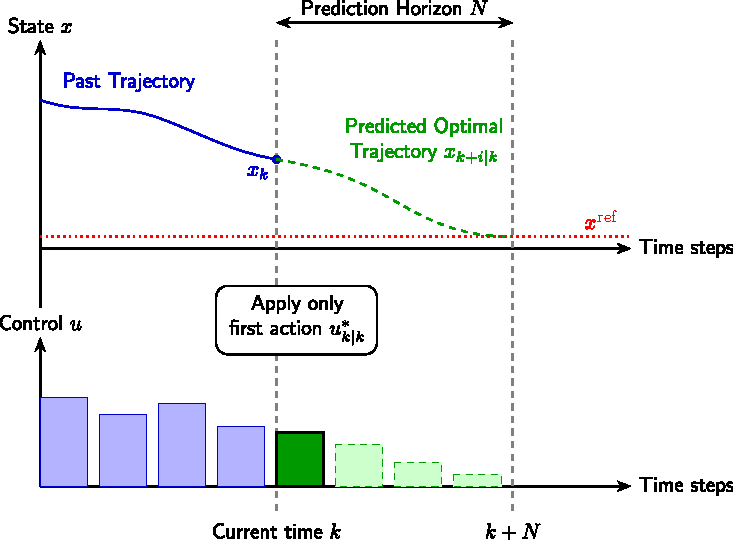
\includegraphics[width=0.9\textwidth]{figs/MPC_Formulation.pdf}
    \caption{Schematic illustrating the MPC strategy. The top graph shows the past trajectory of the system resulting in the current state $x_k$, alongside the predicted optimal trajectory approaching the target $x^{\text{ref}}$ over the prediction horizon $N$. The bottom graph displays the corresponding sequence of calculated control inputs. The fundamental idea behind MPC is to compute full future plan but apply only the immediate action $u^*_{k|k}$.}
    \label{fig:fbd}
\end{figure}
Before we land anything, let us try to understand the mathematical formalism of MPC. Let us consider a system with state $x_k$ (could be the position or momentum or any variable that characterizes the system of interest) at a discrete time $k$. The evolution of the state can be written as $x_{k+1} = F(x_k, u_k)$, where $u_k$ is the control input of the system and $F(x_k, u_k)$ is the process that governs the dynamics of the system. Imagine riding a bicycle, the state $x_k$ describes where you are, how fast you are moving, and in what direction you are moving. The control input $u_k$ is the angle to which you rotate the handlebar or the thrust you provide on the pedal. Those actions determine where you will be in the next instant, which is the new state $x_{k+1}$.

%In the example of landing a rocket, the state may include position, velocity, the amount of fuel left, etc. of the rocket, while the output represents the variables we want to regulate (such as height must go to zero, velocity must go to zero). Now that we have written the system in this form, let us think about what control actually means. At time-step $k$, the state $x_k$ is known. In a traditional feedback setting, we would compute a single input $u_k$ based only on this state and apply it. The system would then move to $x_{k+1}$, and we would repeat the process. 

In the framework of Model Predictive Control, our goal is to decide what is the `best' action to take at a particular instant by considering several future scenarios. That is, at time $k$, we consider a sequence
\[
u_{k|k}, \; u_{k+1|k}, \; u_{k+2|k}, \dots
\]
to choose the control input $u_k$. The notation $u_{k+i|k}$ simply means ``the control input at a future time $k+i$, computed at time $k$''. Once this future input sequence is fixed, the model tells us exactly what will happen next. Using the model $x_{k+1} = F(x_k,u_k)$, we can predict the next state,
\[
x_{k+1|k} = F(x_k, u_{k|k}).
\]
Using the same equation again, we can predict the state two steps ahead,
\[
x_{k+2|k} = F(x_{k+1|k}, u_{k+1|k}).
\]
The state several steps ahead, $x_{k+j|k}$ for $j \gg 1$, depends on the current state, $x_{k|k}$ and on all future control inputs, $u_{k+j|k}$ we have chosen. In other words, once we choose a future control input sequence $u_{k+j|k}$, we have also chosen a future trajectory for the system. Control is not purely reactive, it is about shaping the future trajectory.

The obvious next question is: among all possible future input sequences $u_{k+j|k}$, which one should we choose? To answer this, we introduce a cost function, $J$. The cost function is a measure of how ``good'' a predicted future trajectory is with respect to how we want the system to behave. In the rocket landing example, we want the predicted height and velocity to approach zero over time. At the same time, we do not want to use unnecessarily large thrust. A simple way to express this is to penalize two quantities: the rocket's position error and the control effort. Over a horizon of $N$ future steps, we can define $J$ of the form
\[
J = \lambda_x \sum_{i=1}^{N} \| x_{k+i|k} - x_{k+i}^{\text{ref}} \|^2
+ \lambda_u \sum_{i=0}^{N-1} \| u_{k+i|k} \|^2.
\]
In order to find the control input at time-step $k$, our goal is to minimize $J$ for a fixed horizon $N$. The optimization problem therefore consists of minimizing $J$ over the future input sequence, subject to the dynamic constraint $x_{k+1} = F(x_k, u_k)$. The first term in the cost function $J$ penalizes the deviation from the desired trajectory while the second penalizes excessive control action. Weighting factors $\lambda_{x, u}$ adjust the relative importance of these two objectives. The predicted outputs depend on the chosen input sequence through the system dynamics. If the dynamics is linear and the cost is quadratic, the resulting optimization problem becomes a well known quadratic program. On the other hand, if the dynamics is nonlinear, the optimization becomes a nonlinear program. Therefore, the optimal sequence of inputs can be found by minimizing $J$ with respect to future inputs. The important aspect of MPC compared to other optimal control frameworks is that after computing this optimal control input $u^*_{k+j|k}$ at time-step $k$, we do not apply it for all future times from $k$ to $k+N$, rather we apply only the first control action, $u^*_{k|k}$. At the next time-step, we measure the new state $x_{k+1}$, shift the prediction horizon forward, and solve the optimization problem again. In this way, the control input is continuously re-evaluated based on updated state information. This repeated prediction and optimization is what makes Model Predictive Control adaptive.

In its most general form, a control problem consists of choosing an input sequence $u_k$ that minimizes a performance metric $J(x_k, u_k)$, subject to the system dynamics and physical constraints $x_{k+1} = F(x_k, u_k)$. For a discrete-time system, a finite-horizon optimal control problem can be written as
\[
\min_{\{u_0,\dots,u_{N-1}\}} 
\sum_{k=0}^{N-1} J(x_k, u_k) + \Phi(x_N)
\]
subject to
\[
x_{k+1} = F(x_k, u_k).
\]
Here, $J(x_k,u_k)$ represents the stage cost accumulated at each step and $\Phi(x_N)$ is the terminal cost. Model Predictive Control operates by repeatedly solving such a finite-horizon optimal control problem in real time. At each time-step, the problem is solved using the current state, $x_k$ as the initial condition, the first control action $u_k$ is applied, we shift the horizon ($N$ steps) by one discrete time step $k$ to $k+1$. In this sense, MPC is not a fundamentally different type of controller but rather a real-time implementation of optimal control. With this background in place, let us now try to land the rocket. 

\section*{Landing the Rocket}

\begin{figure}[H]
    \centering
    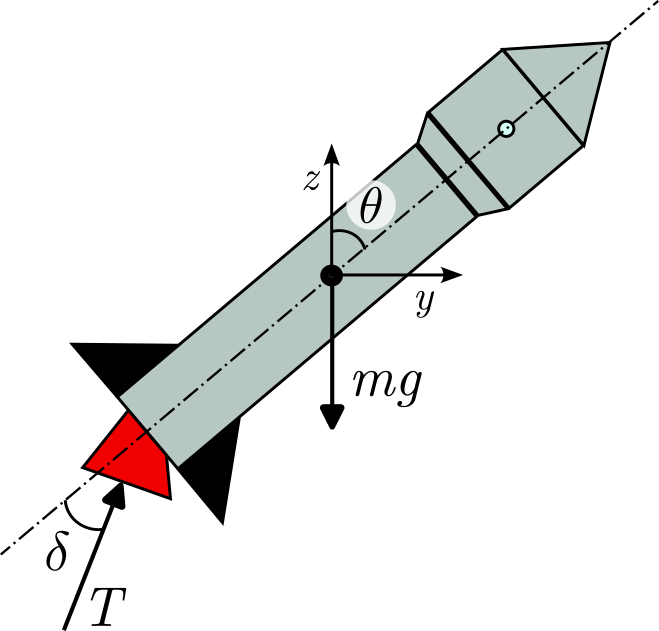
\includegraphics[width=0.35\textwidth]{figs/rocket.png}
    \caption{Schematic of the rocket in the $yz$-plane with its total mass (including fuel) $m$, orientation $\theta$ and control variables, the gimbal angle $\delta$ and the thrust $T$. The mass  of the rocket $m(t)$ evolves with time as the fuel gets consumed to exert thrust $T(t)$ while the gimbal angle $\delta(t)$ can be tuned to change the orientation of the rocket.}
    \label{fig:fbd}
\end{figure}

Consider the task of vertically landing a rocket which, as we shall see, is a concrete instance where we can use the general finite-horizon optimal control framework. Our goal is to plan the motion of a planar rigid rocket with variable mass whose state at time $t$ is given by
\[
\x(t) =
\begin{bmatrix}
y(t) & z(t) & \theta(t) & \dot y(t) & \dot z(t) & \dot \theta(t) & m(t)
\end{bmatrix}^\T,
\]
where $y(t)$ and $z(t)$ denote horizontal and vertical positions, $\theta(t)$ is the pitch angle, $\dot y(t)$, $\dot z(t)$, and $\dot\theta(t)$ are the corresponding velocities, and $m(t)$ is the current mass of the rocket. The control input is
\[
\u(t) =
\begin{bmatrix}
T_{\eff}(t) & \delta(t)
\end{bmatrix}^\T,
\]
where $T_{\eff}(t)$ represents the thrust magnitude and $\delta(t)$ the gimbal deflection angle, which are controlled through actuators. The rocket motion can then be described using Newton's laws for a variable mass rigid body. The thrust acts along the body axis of the rocket, while gravity acts downward (see \ref{fig:fbd} for a schematic of the setup). The translational dynamics is written as
\[
\ddot y = \frac{T_{\mathrm{eff}}}{m} \sin(\theta + \delta),
\qquad
\ddot z = \frac{T_{\eff}}{m} \cos(\theta + \delta) - g.
\]
The thrust exerted by the rocket, $T_{\eff}$ must reach zero when the fuel is empty. This effect is accounted for, while also maintaining the differentiability required by interior-point solvers, by approximating the hard engine cutoff using a smooth function. We define an activation function $\Theta(m)$ that smoothly transitions from $1$ to $0$ as the mass approaches $m_{\text{dry}}$,
\[
\Theta(m) = \frac{1}{2} \left[ 1 + \tanh\big(k (m - m_{\text{dry}})\big) \right],
\]
where $k$ is a steepness parameter that controls the sharpness of the cutoff. The effective thrust is then defined as the commanded thrust scaled by this activation factor,
\[
T_{\text{eff}}(T, m) = T \Theta(m).
\]
The mass depletion dynamics can be written as a single continuous equation,
\[
\dot m = - \frac{T_{\text{eff}}(T, m)}{v_e}.
\]
The translational dynamics driven by this effective thrust are given by
\[
\ddot y = \frac{T_{\text{eff}}(T, m)}{m} \sin(\theta + \delta),
\qquad
\ddot z = \frac{T_{\text{eff}}(T, m)}{m} \cos(\theta + \delta) - g,
\]
and the balance of torque about the center of mass yields the rotational dynamics,
\[
\ddot{\theta} = \frac{\ell_{\text{eff}}(m)}{I(m)} \, T_{\text{eff}}(T, m) \sin(\delta).
\]
These equations define a nonlinear continuous-time model $\dot \x = \mathbf{f}(\x, \u)$. To use this model to perform the landing task using MPC, we need to discretize the temporal dynamics using a numerical scheme such as the 4-th order Runge Kutta scheme. This produces a discrete mapping $\x_{k+1} = \mathbf{F}(\x_k, \u_k)$ given the current state $\x_k$ and the control input $\u_k$. With the model in place, we now identify a cost function that measures performance. For soft landing, position, velocity, and orientation should approach zero near the landing pad. Using the discrete definition of the state,
\[
\x_k =
\begin{bmatrix}
y_k & z_k & \theta_k & \dot y_k & \dot z_k & \dot \theta_k & m_k 
\end{bmatrix}^\T,
\]
a reasonable choice of cost function $J(\x_k, \u_k)$ is
\begin{align*}
J(\x_k, \u_k) =&\
\sum_{k=0}^{N-1}
\bigg[
(\x_k - \x_{\text{target}})^\T Q (\x_k - \x_{\text{target}})
+ W_T T_k \\
&\ + R_T T_k^2
+ R_\delta \delta_k^2
\bigg] + (\x_N - \x_{\text{target}})^\T P (\x_N - \x_{\text{target}}).
\end{align*}
The quadratic term $(\x_k - \x_{\text{target}})^\T Q (\x_k - \x_{\text{target}})$ penalizes deviation from the desired landing state, ensuring that position, velocity, and orientation approach zero. The terminal cost {$(\x_N - \x_{\text{target}})^\T P (\x_N - \x_{\text{target}})$ enforces the accuracy in the final time step. The term $R_T T_k^2$ penalizes large thrust magnitudes, encouraging smoother control inputs, avoiding aggressive actuation. In addition to this, the linear term $W_T T_k$ directly penalizes the total thrust usage. While the quadratic term discourages large instantaneous thrust, the linear term discourages sustained thrust over time, thereby promoting fuel efficient trajectories. 

With the dynamics, cost, and constraints defined, we can now state the landing task explicitly as a finite horizon optimal control problem,
\[
\min_{\{\x_k, \u_k\}} J (\x_k, \u_k)
\]
subject to
\[
\x_{k+1} = \mathbf{F}(\x_k, \u_k), \quad k=0,\dots,N-1,
\]
\[
\x_0 = \x_{\text{measured}},
\]
\[
0 \le T_k \le T_{\max}, \qquad |\delta_k| \le \delta_{\max},
\]
\[
z_k \ge 0, \qquad m_{\text{dry}} \le m_k \le m_{\text{wet}}.
\]
Here, the mass is not directly penalized in the tracking term; fuel efficiency is encouraged through the thrust penalty instead. Solving this problem at each time-step, applying only the first control input, and then repeating the procedure with the updated state yields a receding horizon controller capable of guiding the rocket toward a soft landing while reacting to disturbances along the way. The animation above shows the soft-landing of the rocket using this procedure. The \texttt{python}-code used to generate this animation is available \href{https://github.com/sgangaprasath/MPCTutorial/blob/main/CasADi/RocketMPC.py}{here}. This toy model was inspired by the problem set in Robert Stengel's book on Optimal Control and Estimation.
\subsection*{Computational Implementation}

Translating the continuous-time optimal control problem into code requires a self-consistent discretization procedure. We discretize the dynamics using a 4th-order Runge-Kutta (RK4) scheme with a time step of $dt = 0.1$ s and a horizon of $N = 40$ steps (a 4 sec look-ahead). The resulting Nonlinear Program (NLP) is formulated using \texttt{CasADi} library in python. At each time-step, the NLP is solved using \texttt{IPOPT} and the solver simultaneously optimizes the physical states $\x_k$, controls $\u_k$ and the Lagrange multipliers that ensure $\x_{k+1} = \mathbf{F}(\x_k, \u_k)$ and thrust limits. To achieve real-time feasibility, we use \textit{warm starting}, where we take the optimal control sequence computed at the previous step as the initial guess:
\[
\u^*_{k} = \{ \u_{k|k}, \u_{k+1|k}, \dots, \u_{k+N-1|k} \}
\]
We shift this sequence forward by one step and duplicate the final input to create our initial guess:
\[
\u^{\text{guess}}_{k+1} = \{ \u_{k+1|k}, \u_{k+2|k}, \dots, \u_{k+N-1|k}, \u_{k+N-1|k} \}
\]
We also apply the same shift to the state trajectory $\x_k$ and the lagrange multipliers. This guess places the solver close to the next optimal solution, reducing the computation time and allowing the MPC to run dynamically in real time.

\subsection*{Conclusion}
Model Predictive Control extends the capabilities of optimal control but with added adaptability. At every time-step, we use a model of the system to predict how the future might unfold, choose the sequence of inputs that best balances performance and effort, apply only the first input, and then repeat the process with new information. The primary advantage compared to a fixed controller obtained via an optimal control procedure is that you allow the environmental perturbations to affect the system dynamically and adapt to it with an updated controller. The rocket landing problem is only a toy example; however, the MPC framework is general enough that it is today applied in chemical industry, autonomous vehicle planning, active suspension systems, motor drives, wind turbines and wind farm clusters, and several other places.
\end{document}